\section{Introduction}

Tool-using agents interact with and modify external environments through tool invocations \citep{toolformer23shick}, such as executing code \citep{sweagent24yang, skyrl25cao}, legal complaint drafting, managing customer accounts, or placing orders \citep{lmars25wang, crmweaver25lai, fama25yan}. Unlike standard input-output systems, tool-using agents operate through multi-step actions that evolve the world state, making evaluation dependent not on any single response but on the cumulative effect of the entire interaction \citep{yehudai2025surveyevaluationllmbasedagents}. A natural evaluation paradigm, adopted by benchmarks such as $\tau$-Bench \citep{taubench_24_yao, tau2barres}, is final-state evaluation: a task is solved if the world state at termination matches a target state induced by a gold tool-call sequence.
Constructing benchmarks under this paradigm is particularly demanding. Authoring even a single task involves writing natural-language instructions, configuring the environment, deriving the correct sequence of tool calls, and verifying that the target state is both consistent and reachable \citep{saber2025cuadron, bestpractices2025Zhu}. At the same time, agent capabilities are advancing rapidly, and leading models are approaching the ceiling of existing benchmarks \citep{yehudai2025surveyevaluationllmbasedagents, taubench_24_yao, tau2barres, toolllm24qin, bfcl_25_patil, webarena_24_zhou, swebench_24_Jimenez}. 

The combination of costly manual construction and accelerating saturation creates an urgent need for automatic benchmark generation \citep{autocodebench25chou, deepscholarbench25patel}. However, effective automation first requires identifying the properties a good benchmark should satisfy and how to measure them. Our paper begins by proposing three desiderata for benchmarks of tool-using agents. \emph{Validity} requires every task to be both automatically verifiable and correct in that the gold final state is reachable from the task specification. \emph{Difficulty} requires tasks to meaningfully separate agents of different capability levels. \emph{Coverage} requires benchmark tasks to span structurally diverse patterns of tool use rather than oversampling redundant scenarios. Among these three, coverage has received the least attention and lacks a clear operationalization \citep{Mohammadi_survery_2025}. In this paper, we define it through the lens of tool sequences: the ordered list of tool names in the gold trajectory leading to the target state. Framing coverage in terms of tool sequences also opens a constructive pathway: if the space of valid tool sequences can be explored and sampled directly, it becomes possible to design an automatic method for task generation that explicitly targets all three desiderata. 

\begin{figure*}[!t]
    \centering
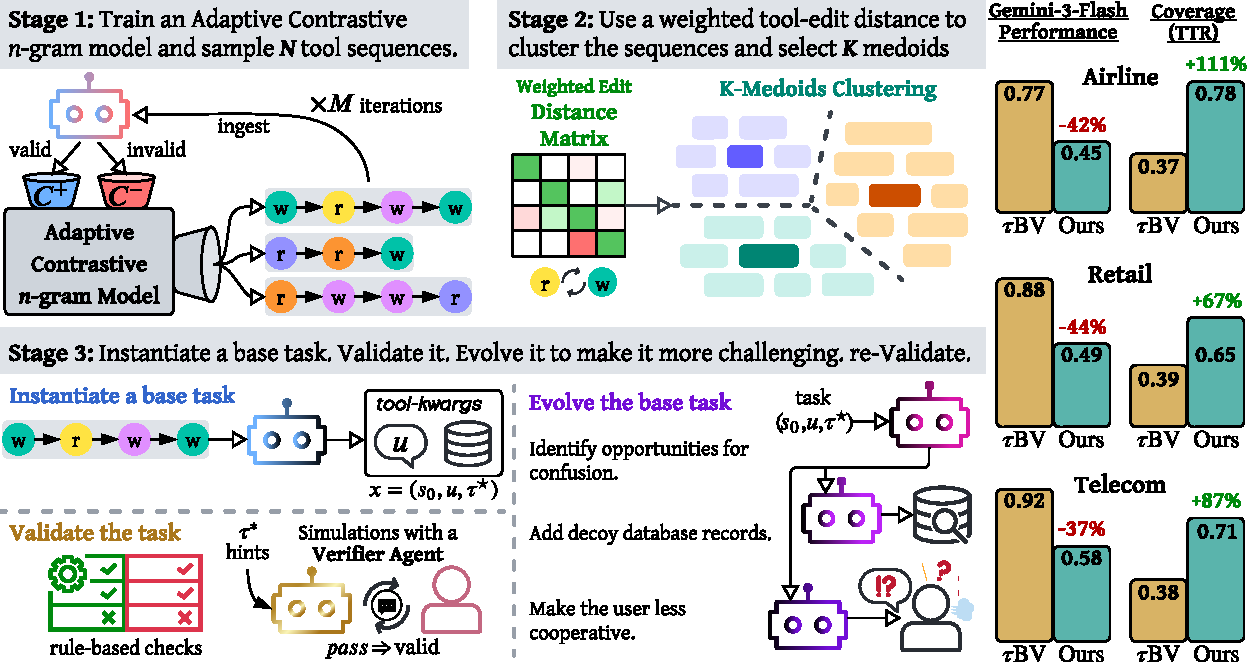
\includegraphics[width=0.98\textwidth]{assets/figures/agents2.pdf}
    \caption{Illustration of TASTE, our three-stage method for synthetic task generation. We demonstrate the method across the three domains of $\tau^2$-Bench (Verified, $\tau\text{BV}$). Evaluating a Gemini-3-Flash agent (averaged over two different user LLMs) shows that, unlike $\tau\text{BV}$, \ourbenchmark is non-saturated. Besides being more challenging, \ourbenchmark exhibits broader coverage, requiring agents to exercise a more diverse set of tool combinations, as quantified by the type-token ratio (TTR; see \S\ref{sec:results}). }
    \label{fig:introfig}
    \vspace{-0.8em}
\end{figure*}

We propose to reverse the task construction process entirely. The prevailing approach involves an author who first writes a natural-language scenario and then derives the corresponding tool sequence. Because the tool-sequence space is never explicitly explored, the resulting benchmarks exercise only arbitrary tool combinations that vary with author choice \citep{Mohammadi_survery_2025}. Accordingly, rather than starting from scenarios and recovering tool sequences, we sample a diverse set of tool sequences and synthesize the full tasks around them. We instantiate this idea and propose \emph{TASTE (\textbf{Ta}sk \textbf{S}ynthesis from \textbf{T}ool Sequence \textbf{E}volution)}, an automatic method for task generation comprising three stages, each targeting one or more of these desiderata. TASTE is illustrated in Figure~\ref{fig:introfig}. 

In the first stage, we train an Adaptive Contrastive $n$-gram model over the space of tool sequences. The model maintains separate count tables for $n$-grams (units are tools) observed in plausibly valid and implausibly valid sequences, as judged by an LLM, and computes sampling probabilities from their contrastive ratio. Counts are updated online through iterative sample-and-validate loops, progressively refining the distribution. This targets \emph{validity} by concentrating probability mass on valid tool sequences, and \emph{coverage} by exploring regions of the tool-combination space.
The second stage selects a representative subset of $K$ (the benchmark size) sequences from the sampled pool using $K$-medoids clustering \citep{kmedoids}. We employ a weighted Levenshtein distance that reflects semantic and functional similarity between tools.
In the third stage, each selected tool sequence is instantiated into a complete benchmark task (user instruction, database records, tool arguments).
Following rule-based checks, we employ a hint-assisted verifier agent to ensure the task is actually solvable: we provide a corrupted version of the gold tool-call sequence (tools are shuffled, arguments are masked), requiring the agent to cooperate with the simulated user to reach the target state. 
A final evolution step targets \emph{interaction difficulty}: making the user ambiguous and less cooperative, and introducing confusing decoy records to the database (e.g., a fully booked flight on the desired route).

Using TASTE, we construct \ourbenchmark, a challenging extension of the three domains of \taubench \citep{tau2barres}: Airline, Retail, and Telecom ($K\!=50\!/114\!/114$ respectively). We then evaluate 11 agent/user LLM pairs across all three domains. We find performance on our \ourbenchmark is consistently and substantially lower than on the original \taubench, with agents scoring up to $80\%$ worse. The degradation is particularly striking for models that appear to have nearly saturated the \taubench: Gemini-3-Flash achieves $0.82\!-\!0.94$ on the original yet drops to $0.28\!-\!0.61$ on ours. Beyond increased difficulty, our benchmark more than doubles the number of unique tool combinations agents must execute: the weighted edit distance between sequences rises by up to $124\%$, the type-token ratio (TTR, the proportion of unique $n$-grams) by up to $111\%$, and tool-frequency entropy by $35\%$. These results suggest that high scores on existing benchmarks often reflect saturation rather than robust task-solving ability, underscoring the need for automated methods like \ourbenchmark that can continuously generate harder tasks with broader coverage.

To summarize, our contributions are as follows:
(1) We articulate three desiderata for benchmarks of tool-using agents: \emph{validity}, \emph{difficulty}, and \emph{coverage}. We further operationalize coverage through tool sequences.
(2) We propose TASTE, a method for automatic task generation that enables exploration of the tool-sequence space.
(3) We construct \ourbenchmark, a challenging extension of \taubench, evaluate it on 11 agent/user LLM pairs, and demonstrate that \ourbenchmark is harder and provides broader coverage of tool-use patterns.
